%# -*- coding: utf-8-unix -*-
% !TEX program = xelatex
% !TEX root = ../main.tex
% !TEX encoding = UTF-8 Unicode
\chapter{Finit Markov Decision Process}
\label{chap:ch_3_Finit_Markov_Decision_Process}

\section{The Agent-Environment Interface}
\begin{enumerate}
    \item \textbf{finite MDP:} the sets of states, actions and rewards($\mathcal{S, A, R}$) all have a finite number of elements.

    \item \textbf{Markov property:} In this case, the random variables $R_t$ and $S_t$ have well defined discrete probability distributions dependent only on the preceding state and action.
    \begin{equation}
        p(s', r|s, a) \dot{=} Pr\{S_t=s', R_t=r|S_{t-1}=s, A_{t-1}=a\}
    \end{equation}

    \item \textbf{state-transitation probabilities:}
    \begin{equation}
        p(s'|s,a) \dot{=} Pr\{S_t=s'|S_{t-1}=s, A_{t-1}=a\} = \sum_{r \in \mathcal{R}}p(s',r|s,a)
    \end{equation}

    \item \textbf{expected rewards for state–action pairs:}
    \begin{equation}
        r(s,a) \dot{=} \mathbb{E}[R_t|S_{t-1}=s, A_{t-1}=a] = \sum_{r \in \mathcal{R}}r\sum_{s' \in \mathcal{S}}p(s',r|s, a)
    \end{equation}

    \item \textbf{expected rewards for state-action-next-state triplets:}
    \begin{equation}
        r(s,a,s') \dot{=} \mathbb{E}[R_t|S_{t-1}=s,A_{t-1}=a, S_t=s']=\sum_{r \in \mathcal{R}}r\frac{p(s',r, s, a)}{p(s'|s,a)}
    \end{equation}
\end{enumerate}

\section{Goals and Rewards}
\textbf{Reward hypothesis}:That all of what we mean by goals and purposes can be well thought of as the maximization of the expected value of the \textbf{cumulative sum of a received scalar signal} (called reward).

\section{Returns and Episodes}
\begin{enumerate}
    \item \textbf{episodic(episode) tasks:} when the agent–environment interaction breaks naturally into subsequences, which we call episodes. Tasks with episodes of this kind are called episodic tasks.

    \item \textbf{continuing tasks:} the agent–environment interaction does not break naturally into identifiable episodes, but goes on continually without limit.

    \item \textbf{return(simple):}
        \begin{equation}
            G_t \dot{=} R_{t+1}+R_{t+2}+R_{t+3}+\dots+R_T
        \end{equation}

    \item \textbf{discounted return:}
        \begin{equation}
            G_t \dot{=} R_{t+1}+ \gamma R_{t+2} + \gamma^2 R_{t+3} + \dots = \sum_{k=0}^{\infty}\gamma^kR_{t+k+1}
        \end{equation}
    where $\gamma$ is a parameter, $0 \leq \gamma \leq 1$, called the \textbf{discount rate}. As $\gamma$ approaches 1, the return objective takes future rewards into account more strongly; the agent becomes more farsighted.

    \item \textbf{Returns at successive time steps:}
        \begin{equation}
        \begin{split}
            G_t \dot{=} & R_{t+1}+\gamma R_{t+2}+\gamma^2 R_{t+3} + \gamma^3 R_{t+4}+\dots\\
                = &R_{t+1} + \gamma (R_{t+2}+\gamma^1 R_{t+3} + \gamma^2 R_{t+4}+\dots)\\
                = &R_{t+1} + \gamma G_{t+1}
        \end{split}
        \end{equation}

\end{enumerate}

\section{Unified Notation for Episodic and Continuing Tasks}

\section{Policies and Value Functions}
\begin{enumerate}
    \item \textbf{policy:} a mapping from states to probabilities of selecting each possible action. If the agent is following policy $\pi$ at time $t$ , then $\pi(a|s)$ is the probability that $A_t = a$ if $S_t = s$.

    \item \textbf{state-value function for policy $\pi$:} the expected return when starting in $s$ and following $\pi$ thereafter:
        \begin{equation}
            v_{\pi}(s) \dot{=} \mathbb{E}_{\pi}[G_t|S_t=s] \quad \forall s \in \mathcal{S}
        \end{equation}

    \item \textbf{action-value function for policy $\pi$:} the expected return starting from $s$ , taking the action $a$ , and thereafter following policy $\pi$:
        \begin{equation}
            q_{\pi}(s,a) \dot{=} \mathbb{E}_{\pi}[G_t|S_t=s, A_t=a]
        \end{equation}

    \item \textbf{$v_{\pi}(s)$ vs $q_{\pi}(s,a)$:}
        \begin{equation}
            v_{\pi}(s) = \sum_{a \in \mathcal{A}}\pi(a|s)q_{\pi}(s,a)
        \end{equation}

    \item \textbf{Bellman equation for $v_{\pi}$:} It states that the value of the start state must equal the (discounted) value of the expected next state, plus the reward expected along the way. as show in Figure-\ref{fig:dackup_diagram_for_vpi}
        \begin{equation}
        \begin{split}
            v_{\pi}(s) \dot{=} & \mathbb{E}_{\pi}[G_t|S_t=s]\\
                = & \mathbb{E}_{\pi}[R_{t+1}+\gamma G_{t+1}|S_t=s]\\
                = & \sum_{a}\pi(a|s)\sum_{s'}\sum_{r}p(s',r|s,a)[r+\gamma \mathbb{E}_{\pi}[G_{t+1}|S_{t+1}=s']]\\
                = & \sum_{a}\pi(a|s)\sum_{s', r}p(s',r|s,a)[r+\gamma v_{\pi}(s')]
        \end{split}
        \end{equation}

    \item \textbf{Bellman equation for $q_{\pi}$:}

        \begin{equation}
        \begin{split}
            q_{\pi}(s,a) = & \sum_{s'} \sum_{r} p(s', r|s,a)[r+ \gamma v_{\pi}(s')] \\
                = & \sum_{s'}\sum_{r}p(s', r|s, a)[r+ \gamma \sum_{a'} \pi (a'|s') q_{\pi}(s',a')]
        \end{split}
        \end{equation}

    \item \textbf{$q_{\pi}(s,a)$ vs $v_{\pi}(s')$:}
        \begin{equation}
            q_{\pi}(s,a) =  \sum_{s'} \sum_{r} p(s', r|s,a)[r+ \gamma v_{\pi}(s')]
        \end{equation}
\end{enumerate}

\begin{figure}[htbp]
    \centering
    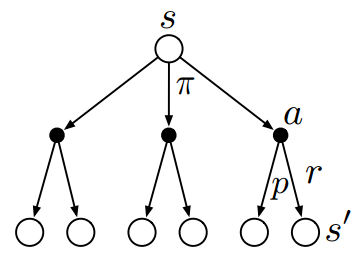
\includegraphics[width=0.3\textwidth]{figs/ch_3_5_1_dackup_diagram_for_vpi.png} 
    \caption{Backup diagram for $v_{\pi}$}
    \label{fig:dackup_diagram_for_vpi}
\end{figure}

\section{Optimal Policies and Optimal Value Functions}
\begin{enumerate}
    \item \textbf{optimal policy:} A policy $\pi$ is defined to be better than or equal to a policy $\pi '$ if its expected return is greater than or equal to that of $\pi '$ for all states. In other words, $\pi \geq \pi '$ if and only if $v_{\pi}(s) \geq v_{\pi '}$ for all $s \in \mathcal{S}$. There is always at least one policy that is better than or equal to all other policies. This is an optimal policy $\pi_{*}$.

    \item \textbf{optimal state-value function:} 
        \begin{equation}
            v_{*}(s) \dot{=} \max_{\pi} v_{\pi}(s) \quad \forall s \in \mathcal{S}
        \end{equation}

    \item \textbf{optimal action-value function:}
        \begin{equation}
            q_{*}(s,a) \dot{=} \max_{\pi} q_{\pi}(s, a) \quad \forall s \in \mathcal{S} \quad and \quad \forall a \in \mathcal{A}(s)        
        \end{equation}
    For the state-action pair $(s, a)$, this function gives the expected return for taking action $a$ in state $s$ and thereafter following an optimal policy.
        \begin{equation}
            q_{*}(s,a) = \mathbb{E}[R_{t+1} + \gamma v_{*}(S_{t+1})|S_t=s, A_t=a]
        \end{equation}

    \item \textbf{Bellman optimality equation for $v_*$:} Intuitively, the Bellman optimality equation expresses the fact that the value of a state under an optimal policy must equal the expected return for the best action from that state. As show in Figure-\ref{fig:backup_diagrams_v_and_q}
    \begin{equation}
    \begin{split}
        v_*(s) = & \max_{a \in \mathcal{A}(s)} q_{\pi_*}(s,a) \\
            = & \max_a \mathbb{E}_{\pi_*}[G_t|S_t=s, A_t=a] \\
            = & \max_a \mathbb{E}_{\pi_*}[R_{t+1} + \gamma G_{t+1}|S_t=s,A_t=a] \\
            = & \max_a \mathbb{E}[R_{t+1} + \gamma v_*(S_{t+1})|S_t=s, A_t=a] \\
            = & \max_a \sum_{s', r} p(s',r|s,a)[r + \gamma v_*(s')]
    \end{split}
    \end{equation}

    \item \textbf{Bellman optimality equation for $q_*$:} As show in Figure-\ref{fig:backup_diagrams_v_and_q}
    \begin{equation}
    \label{eq:bellman_optimality_equation}
    \begin{split}
        q_*(s,a) = & \mathbb{E}[R_{t+1} + \gamma v_*(S_{t+1})|S_t=s, A_t=a] \\
            = & \mathbb{E}[R_{t+1} + \gamma \max_{a'}q_*(S_{t+1}, a')| S_t=s, A_t=a] \\
            = & \sum_{s',r} p(s',r|s, a)[r+ \gamma \max_{a'}q_*(s', a')]
    \end{split}
    \end{equation}
\end{enumerate}
\begin{figure}[htbp]
    \centering
    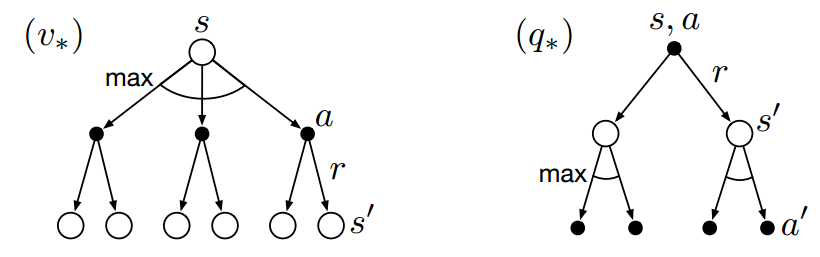
\includegraphics[width=0.6\textwidth]{figs/ch_3_6_1_backup_diagrams_v_and_q.png} 
    \caption{Backup diagram for $v_{*}$ and $q_{*}$}
    \label{fig:backup_diagrams_v_and_q}
\end{figure}
